\documentclass[../main.tex]{subfiles}

\begin{document}

\begin{definition}
A filtered chain complex $C_*$ is a chain complex with a filtration
\[\cdots\to F_{p-1}C_*\to F_pC_*\to F_{p+1}C_*\to\cdots\to C_*\]
Where $F_pC_*$ are chain complexes, and the maps are chain maps, more concretely
\begin{center}
\begin{tikzcd}
                 & \vdots                             & \vdots                           & \vdots                             &                  & \vdots            \\
\cdots \arrow[r] & F_{p-1}C_{i+1} \arrow[r] \arrow[u] & F_{p}C_{i+1} \arrow[r] \arrow[u] & F_{p+1}C_{i+1} \arrow[r] \arrow[u] & \cdots \arrow[r] & C_{i+1} \arrow[u] \\
\cdots \arrow[r] & F_{p-1}C_{i} \arrow[r] \arrow[u]   & F_{p}C_{i} \arrow[r] \arrow[u]   & F_{p+1}C_{i} \arrow[r] \arrow[u]   & \cdots \arrow[r] & C_i \arrow[u]     \\
\cdots \arrow[r] & F_{p-1}C_{i-1} \arrow[r] \arrow[u] & F_{p}C_{i-1} \arrow[r] \arrow[u] & F_{p+1}C_{i-1} \arrow[r] \arrow[u] & \cdots \arrow[r] & C_{i-1} \arrow[u] \\
                 & \vdots \arrow[u]                   & \vdots \arrow[u]                 & \vdots \arrow[u]                   &                  & \vdots \arrow[u] 
\end{tikzcd}
\end{center}
\end{definition}

\begin{example}
Tuple chain complex $C_*(X)$ in Definition \ref{Definition of tuple chain complex} is a filtered chain complex with filtration
\[\cdots\to C^{p-1}_*(X)\to C^{p}_*(X)\to C^{p+1}_*(X)\to\cdots\to C_*(X)\]
If $X$ is a topological space with a filtrations of subspaces(CW complex with skeletons is a special case)
\[\cdots\subseteq X^{p-1}\subseteq X^p\subseteq X^{p+1}\subseteq X\]
Then the singular chain complex $C^{\mathrm{sing}}_*(X)$ is a filtered chain complex with filtration
\[\cdots\to C_*(X^{p-1})\to C_*(X^{p})\to C_*(X^{p+1})\to\cdots\to C_*(X)\]
\end{example}

\begin{definition}
Suppose $R$ is a commutative ring with identity \par
A \textbf{graded module}\index{Graded module} is a module with grading $A=\bigoplus_{n}A_n$, $n\in I$ is a totally ordered set, mostly we just consider $\mathbb Z$ \par
A \textbf{filtered module}\index{Filtered module} is a module with a filtration
\[\cdots\hookrightarrow F_{p-1}A\hookrightarrow F_pA\hookrightarrow F_{p+1}A\hookrightarrow\cdots\hookrightarrow A\]
We can define the graded module associated to the filtration $grA=\bigoplus_p F_{p+1}A/F_pA$ \par
A \textbf{filtered graded module}\index{Filtered graded module} is a graded module $A=\bigoplus_{n}A_n$ with a filtration of graded modules
\[\cdots\hookrightarrow F_{p-1}A\hookrightarrow F_pA\hookrightarrow F_{p+1}A\hookrightarrow\cdots\hookrightarrow A\]
Such that filtration preserving grading, i.e. $\displaystyle F_pA\subseteq\bigoplus_{n\leq p}A_n$, then we have
\[\displaystyle F_pA=F_pA\bigcap\bigoplus_{n\leq p}A_n=\bigoplus_{n\leq p}F_pA\cap A_n\]
Define $(F_pA)_n$ or $F_pA_n:=F_pA\cap A_n$, then
\[\cdots\hookrightarrow F_{p-1}A_n\hookrightarrow F_{p}A_n\hookrightarrow F_{p+1}A_n\hookrightarrow\cdots\hookrightarrow A_n\]
Is a filtration of $A_n$, and $(F_pA)_n$ are the direct summands of $F_pA$, we also have a grid
\begin{center}
\begin{tikzcd}
\cdots \arrow[r, hook] & F_{p-1}A \arrow[r, hook]                       & F_{p}A \arrow[r, hook]                       & F_{p+1}A \arrow[r, hook]                       & \cdots \arrow[r, hook] & A                       \\
                       & \vdots \arrow[u, hook]                         & \vdots \arrow[u, hook]                       & \vdots \arrow[u, hook]                         &                        & \vdots \arrow[u, hook]  \\
\cdots \arrow[r, hook] & F_{p-1}A_{i+1} \arrow[r, hook] \arrow[u, hook] & F_{p}A_{i+1} \arrow[r, hook] \arrow[u, hook] & F_{p+1}A_{i+1} \arrow[r, hook] \arrow[u, hook] & \cdots \arrow[r, hook] & A_{i+1} \arrow[u, hook] \\
\cdots \arrow[r, hook] & F_{p-1}A_{i} \arrow[r, hook] \arrow[u, hook]   & F_{p}A_{i} \arrow[r, hook] \arrow[u, hook]   & F_{p+1}A_{i} \arrow[r, hook] \arrow[u, hook]   & \cdots \arrow[r, hook] & A_i \arrow[u, hook]     \\
\cdots \arrow[r, hook] & F_{p-1}A_{i-1} \arrow[u, hook] \arrow[r, hook] & F_{p}A_{i-1} \arrow[u, hook] \arrow[r, hook] & F_{p+1}A_{i-1} \arrow[u, hook] \arrow[r, hook] & \cdots \arrow[r, hook] & A_{i-1} \arrow[u, hook] \\
                       & \vdots \arrow[u, hook]                         & \vdots \arrow[u, hook]                       & \vdots \arrow[u, hook]                         &                        & \vdots \arrow[u, hook] 
\end{tikzcd}
\end{center}
\end{definition}

\begin{example}
Let $C_*$ be a filtered chain complex, the homology $\displaystyle H_*C=\bigoplus_{p}H_pC$ is a graded graded module with filtration with $F_pH_nC=\mathrm{im}(H_n(F_pC)\to H_*C)$
\end{example}

\begin{definition}
A \textbf{spectral sequence}\index{Spectral sequence} is a sequence of bigraded module $\{E^r_{*,*}\}$ together with differentials $\partial_{p,q}^r:E^r_{p,q}\to E^r_{p-r,q+r-1}$ such that $\partial^r\circ\partial^r=0$ and $E^{r+1}\cong\ker\partial^r/\mathrm{im}\partial^r=:Z^r/B^r$, $E^r$ are called the $r$-th page
\begin{center}
\begin{tikzpicture}[scale=0.7]
\draw[->](-1,0)--(6,0);
\draw[->](0,-1)--(0,6);
\foreach \x in {0,1,...,5}
{
\foreach \y in {0,1,...,5}
{
\filldraw (\x,\y) circle (0.02);
}
}
\node at (-1,6) {$E^0$};
\foreach \x in {1,...,5}
{
\foreach \y in {1,...,5}
{
\draw[red,->] ($(\x,\y)+0.1*(0,-1)$)--($(\x,\y-1)-0.1*(0,-1)$);
}
}
\end{tikzpicture}
\begin{tikzpicture}[scale=0.7]
\draw[->](-1,0)--(6,0);
\draw[->](0,-1)--(0,6);
\foreach \x in {0,1,...,5}
{
\foreach \y in {0,1,...,5}
{
\filldraw (\x,\y) circle (0.02);
}
}
\node at (-1,6) {$E^1$};
\foreach \x in {1,...,5}
{
\foreach \y in {1,...,5}
{
\draw[red,->] ($(\x,\y)+0.1*(-1,0)$)--($(\x-1,\y)-0.1*(-1,0)$);
}
}
\end{tikzpicture}
\end{center}
\begin{center}
\begin{tikzpicture}[scale=0.7]
\draw[->](-1,0)--(6,0);
\draw[->](0,-1)--(0,6);
\foreach \x in {0,1,...,5}
{
\foreach \y in {0,1,...,5}
{
\filldraw (\x,\y) circle (0.02);
}
}
\node at (-1,6) {$E^2$};
\foreach \x in {2,...,5}
{
\foreach \y in {1,...,4}
{
\draw[red,->] ($(\x,\y)+0.1*(-2,1)$)--($(\x-2,\y+1)-0.1*(-2,1)$);
}
}
\end{tikzpicture}
\begin{tikzpicture}[scale=0.7]
\draw[->](-1,0)--(6,0);
\draw[->](0,-1)--(0,6);
\foreach \x in {0,1,...,5}
{
\foreach \y in {0,1,...,5}
{
\filldraw (\x,\y) circle (0.02);
}
}
\node at (-1,6) {$E^3$};
\foreach \x in {3,...,5}
{
\foreach \y in {1,...,3}
{
\draw[red,->] ($(\x,\y)+0.1*(-3,2)$)--($(\x-3,\y+2)-0.1*(-3,2)$);
}
}
\end{tikzpicture}
\end{center}
Since $Z^{i+1},B^{i+1}$ are submodules of $Z^i/B^i$, we have
\[\cdots\subseteq B^i\subseteq B^{i+1}\subseteq\cdots\subseteq Z^{i+1}\subseteq Z^i\subseteq\cdots\]
Define $B^\infty=\bigcup_r B^r$, $Z^\infty=\bigcap_r Z^r$, $E^\infty=Z^\infty/B^\infty$
\end{definition}

\begin{definition}
A spectral sequence converges to a filtered graded module $A$ if $E^\infty_{p,q}=F_pA_{p+q}/F_{p-1}A_{p+q}$, or equivalently $\displaystyle\bigoplus_{p+q=n}E^n_{p,q}=grA_n$, we write as $E_{p,q}^1\Rightarrow A_{p+q}$
\begin{center}
\begin{tikzpicture}[scale=0.5]
\draw[->](-1,0)--(6,0);
\draw[->](0,-1)--(0,6);
\foreach \x in {0,1,...,5}
{
\foreach \y in {0,1,...,5}
{
\filldraw (\x,\y) circle (0.02);
}
}
\node[above] at (-1,6) {$E^\infty$};
\draw(-1,6)--(6,-1);
\node[below] at (6,-1) {$p+q=n$};
\end{tikzpicture}
\end{center}
\end{definition}

\begin{theorem}[Serre spectral sequence]
Let $F\to E\to B$ be a filtration, suppose $\pi_1(B)$ acts on $H_*(F)$ trivially, then there is a spectral sequence with $E^2_{p,q}=H_p(B;H_q(F))\Rightarrow H_{p+q}(E)$, meaning converges to $H_*(E)$
\end{theorem}

\begin{example}[Wang sequence]
Suppose $F\to E\to B$ be a filtration, with $B=S^k$, then $E^2_{p,q}=H_p(B;H_q(F))=H_p(B)\otimes H_q(F)$ by universal coefficient theorem, since $H_p(B)=\begin{cases}
\mathbb Z, &p=0,k \\
0, &\text{Otherwise}
\end{cases}$, we have the second page
\begin{center}
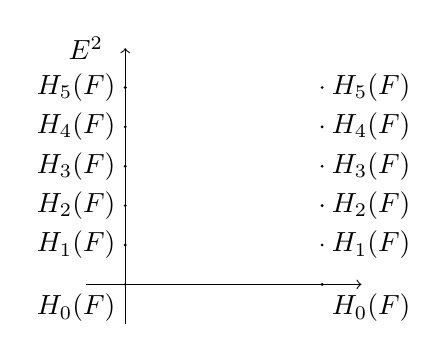
\begin{tikzpicture}[scale=0.5]
\draw[->](-1,0)--(6,0);
\draw[->](0,-1)--(0,6);
\foreach \x in {0,5}
{
\foreach \y in {0,1,...,5}
{
\filldraw (\x,\y) circle (0.02);
}
}
\node at (-1,6) {$E^2$};
\foreach \z in {1,...,5}
{
\node[left] at (0,\z) {$H_{\z}(F)$};
\node[right] at (5,\z) {$H_{\z}(F)$};
}
\node[below left] at (0,0) {$H_{0}(F)$};
\node[below right] at (5,0) {$H_{0}(F)$};
\end{tikzpicture}
\end{center}
The only non trivial differential appears on page $k$, thus we have $E^2=E^3=\cdots=E^k$, $E^{k+1}=E^{k+2}=\cdots=E^\infty$, on page $k$, we have $\partial^k:E^k_{k,r}\to E^k_{0,r+k-1}$, thus $\ker\partial^k=E^{k+1}_{k,r}=E^{\infty}_{k,r}$, $\mathrm{coker}\partial^k=E^{k+1}_{0,r+k-1}=E^{\infty}_{k0,r+k-1}$
\begin{center}
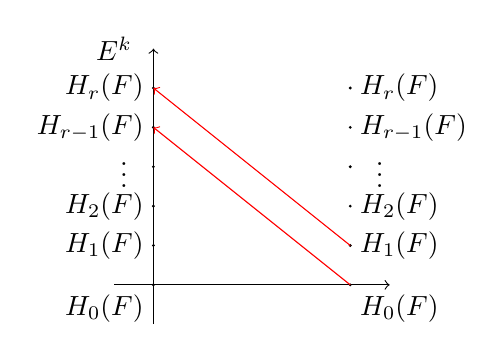
\begin{tikzpicture}[scale=0.5]
\draw[->](-1,0)--(6,0);
\draw[->](0,-1)--(0,6);
\foreach \x in {0,5}
{
\foreach \y in {0,1,...,5}
{
\filldraw (\x,\y) circle (0.02);
}
}
\node at (-1,6) {$E^k$};
\foreach \z in {1,2}
{
\node[left] at (0,\z) {$H_{\z}(F)$};
\node[right] at (5,\z) {$H_{\z}(F)$};
}
\node[below left] at (0,0) {$H_{0}(F)$};
\node[below right] at (5,0) {$H_{0}(F)$};
\node[left] at (-0.4,3) {$\vdots$};
\node[right] at (5.4,3) {$\vdots$};
\node[left] at (0,4) {$H_{r-1}(F)$};
\node[right] at (5,4) {$H_{r-1}(F)$};
\node[left] at (0,5) {$H_{r}(F)$};
\node[right] at (5,5) {$H_{r}(F)$};
\draw[red,->] (5,0)--(0,4);
\draw[red,->] (5,1)--(0,5);
\end{tikzpicture}
\end{center}
Therefore we get an exact sequence
\[0\to E^\infty_{k,r}\to H_r(F)\to H_{r+k-1}(F)\to E^{\infty}_{0,r+k-1}\to0\]
Replace $r$ with $n-k$, we get
\[0\to E^\infty_{k,n-k}\to H_{n-k}(F)\to H_{n-1}(F)\to E^{\infty}_{0,n-1}\to0\]
Since $H_n(E)=E^\infty_{k,n-k}\oplus E^\infty_{0,n}$, there is also an exact sequence
\[0\to E^\infty_{k,n-k}\to H_n(E)\to E^\infty_{0,n}\to0\]
Put them together, we get the \textbf{Wang sequence}\index{Wang sequence}
\[\cdots\to H_n(E)\to H_{n-k}(F)\to H_{n-1}(F)\to H_{n-1}(E)\to\cdots\]
\end{example}

\end{document}